\subsection{Star Decomposition and Matching}\label{sec:match_star}
%% Generally speaking, there are two kinds of graph isomorphism algorithm,
%% differing on whether intermediate results are materialized.
%% The first is the backtracking tree-searching method~\cite{DBLP:journals/jacm/Ullmann76,DBLP:journals/pvldb/LeeHKL12,DBLP:conf/sigmod/HanLL13,DBLP:conf/sigmod/KimLBHLKJ16},
%% which does not generate intermediate results.
%% However, tree-searching algorithms are prone to the random disk access problem since the vertices are scattered among the disk.
%% The second is the join-based algorithm~\cite{DBLP:journals/pvldb/LaiQLC15,DBLP:journals/pvldb/QiaoZC17,DBLP:journals/pvldb/SunWWSL12,DBLP:journals/pvldb/MhedhbiS19},
%% which decomposes the pattern graph into smaller matching units and materialize the intermediate results.
%% The final result is obtained by joining on these intermediate results.
%% In practice, the intermediate results contain valuable information and are cached for queries issued afterward.
%% Based on these observations, SeqStar adopts the join-based approach.


%% Because of the intrinsic poor locality of graphs,
%% tree-based algorithms would incur incredible random disk accesses when jumping between the vertices scattered among the disk.
%% Therefore, a join based matching algorithm is more suitable for real world problems.
%% However, to \emph{choose a proper join unit that can avoid random disk accesses and minimize the intermediate results as well} is still a hard problem.
%% Perhaps the most intuitive way is to decompose the original pattern graph into a series of edges.
%% However, lots of useless intermediate results would be generated by doing so.
%% Consider the diamond pattern graph in Figure~\ref{img:pattern_graph},
%% many intermediate results would be generated if they were matched in Figure~\ref{img:celebrity_star},
%% however, they are all pointless since there is no such a graph that could match the original diamond pattern.
%% To solve this problem, more complex structures such as frequent subgraphs, multi-hop edges could be used,
%% however, as Sun et al\@. have stated before,
%% these methods require complex index that has super-linear space and time complexity~\cite{DBLP:journals/pvldb/SunWWSL12}, and are not very suitable for solving real world property graph matching problems.

%% Recall the vertex-centric property graph storage model that we discussed previously,
%% which provides two efficient iterators that can scan the vertices (via \textsc{VertexIter}) and neighbors (via \textsc{NeighborIter}) sequentially (Section~\ref{sec:storage_iterators}),
%% if the matching process only requires neighborhood link information,
%% random disk accesses could then be avoided.
%% Based on this observation, we make a balance by using stars as our basic matching unit.
%% As is shown in Figure~\ref{img:pattern_graph}, a star graph contains a root vertex and some neighbors connected to the root.
%% The star pattern can then be matched within a sequential disk scan based on our vertex-centric storage model:
%% 1\@. Select the domain of interest using the global index,
%% 2\@. iterate through the relevant vertices by the \textsc{VertexIter},
%% 3\@. and for each visited vertex, use the \textsc{NeighborIter} to check the neighbors to determine whether the star would be matched.
%% Besides, a star contains far more structural information then an edge,
%% which means the matching results of a star have a predictable smaller size.
%% Moreover, we made further contributions to keep the matching results even smaller (Section~\ref{sec:match_compress} and Section~\ref{sec:match_optimize}).

%% Some existing works also adopt star-like structures as their basic matching unit~\cite{DBLP:journals/pvldb/SunWWSL12,DBLP:journals/pvldb/LaiQLC15},
%% however, SeqStar takes further steps in two different ways:
%% \begin{enumerate}[noitemsep,leftmargin=0pt,align=left,labelwidth=\parindent]
%% \item SeqStar adopts the property graph model (Section~\ref{sec:background}) rather than the simple graph model ubiquitous among academical paper.
%%   A simple graph can be viewed as a special case of a property graph,
%%   which ignores the labels, multi-edges, or even the direction of edges.
%%   However, real-world applications of simple graphs are very limited because of the information they dropped out.
%%   It is not easy to make a simple graph matching algorithm to solve the property graph matching problem.
%%   For one thing, it is a hard engineering problem, because the traditional underlying graph storage method is not suitable for property graphs (Section~\ref{sec:storage}).
%%   For another, many existing work rely on the perfect isotropic properties of a simple graph to operate and optimize their algorithms~\cite{DBLP:journals/pvldb/SunWWSL12,DBLP:conf/sigmod/HanLL13,DBLP:journals/pvldb/QiaoZC17}.
SeqStar uses a novel star decomposition algorithm that preserves as much matching information as possible.
It also harness the star isomorphism to scan the graph data sequentially for only once.

%On top of the vertex-centric storage engine, SeqStar reduces the I/O cost by analyzing star isomorphism and scanning the graph data sequentially only once.

Some existing works also adopt star-like structures~\cite{DBLP:journals/pvldb/SunWWSL12,DBLP:journals/pvldb/LaiQLC15}. However, they lose valuable filtering information in stars and result in unnecessary intermediate results.
Consider the pattern graph in Figure~\ref{img:running_example}. $u_1$ and $u_4$ are selected as the roots.
Existing decomposition algorithms~\cite{DBLP:journals/pvldb/SunWWSL12,DBLP:journals/pvldb/LaiQLC15} will generate two stars as shown in Figure~\ref{img:stwig}.
\begin{figure}[ht]
  \centering
  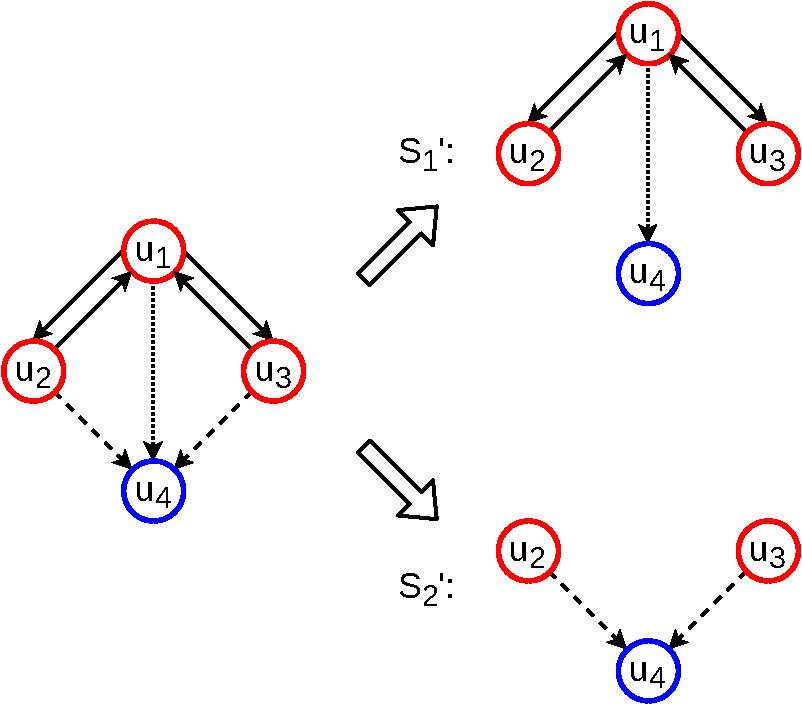
\includegraphics[width=0.35\textwidth]{img/stwig.pdf}
  \caption{Stars generated by existing algorithms.}\label{img:stwig}
\end{figure}
The edge $u_1 \rightarrow u_4$ is lost in $S_2'$.
Therefore, vertex $10$ will be matched (Figure~\ref{img:running_example}) which is unnecessary.
The problem is more severe for complex patterns where more edges need to be discarded.

SeqStar addresses the problem by keeping the original pattern graph unchanged, and removing vertices/edges on a copy $p'$ of the pattern (Algorithm~\ref{alg:decompose_stars}).
Algorithm~\ref{alg:decompose_stars} is similar to the vertex-cover selection algorithm~\cite{DBLP:books/daglib/0023376}.
The set $R$ in Algorithm~\ref{alg:decompose_stars} stores the candidate root vertices.
The algorithm uses a heuristic function: \[f(u) = \frac{\deg(u) + |\psi(u)|}{\operatorname{freq}(u.label)}\] to select roots,
where $\deg(u)$ is the degree of $u$, $|\psi(u)|$ is the number of constraints related to $u$ ($u_2 > u_1$, $u_3 > u_1$, $u_4 < 8$ in Figure~\ref{img:running_example}),
and $\operatorname{freq}(u.label)$ is the frequency of $u$'s label in the data graph.
By maximizing the function $f$,
SeqStar prefers vertex that
(1) has a high degree and has more associated constraints,
(2) has a less popular label in the data graph.
Therefore, the size of intermediate results from star matching can be reduced.
The neighbors of the selected root will then be added to the candidate set $R$.
By doing so, the roots selected by Algorithm~\ref{alg:decompose_stars} will be connected and forms a \emph{connected vertex-cover}.
And we'll use this property to build index for join operations (\S~\ref{sec:match_join}).
Finally, SeqStar uses the selected root to extract stars from the original pattern graph $p$.
$\operatorname{Star}(p, root)$ is obtained by copying all the edges connected with $root$.
Therefore, all the structural information of $p$ is inherited to the stars.
%TODO:这里加讨论,这两条的点在之后的匹配中能够起到什么作用。

  %% Consider the pattern graph in Figure~\ref{img:star_decomposition},
  %% suppose that $u_1$, $u_2$ and $u_3$ are selected as the roots,
  %% existing decomposition method would result in three stars with 3, 2 and 1 neighbor\@(s)
  %% by consecutively selecting and removing vertices from the original pattern.
  %% However, many useful matching information are lost by doing so,
  %% e.g., the third ``star'' is just an edge, which would generate enormous unnecessary matching results whereas every edge in the data graph would match it but only a part of them could match the original pattern graph.
  %% In contrast, our approach (Algorithm~\ref{alg:decompose_stars}) would keep all the neighborhood matching information as is shown in the bottom of Figure~\ref{img:star_decomposition}, which could then reduce unnecessary intermediate results significantly (Section~\ref{sec:experiments}).
  %% Like previous work~\cite{DBLP:journals/pvldb/SunWWSL12}, we also use a heuristic function to select a join order, which is defined as $ f(u) = \frac{\deg(u) + |\psi(u)|}{\operatorname{freq}(u.label)} $, i.e.,
  %% we prefer to select vertex with bigger degree (more early filters) and less label frequency (smaller intermediate matching results) first.
  %% $|\psi(u)|$ is the number of local constraints of $u$, which will be discussed further in Section~\ref{sec:match_optimize}.
  %% The root candidate set $R$ is used to select a connected vertex cover,
  %% which could then be joined efficiently (Section~\ref{sec:match_join}).
  %% The key feature of the algorithm is to remove selected vertex in a copy $p'$ of the pattern and always keeps the original useful information in $p$, and thus, the intermediate results of our star could be much smaller.
  %% \begin{figure}[ht]
  %%   \centering
  %%   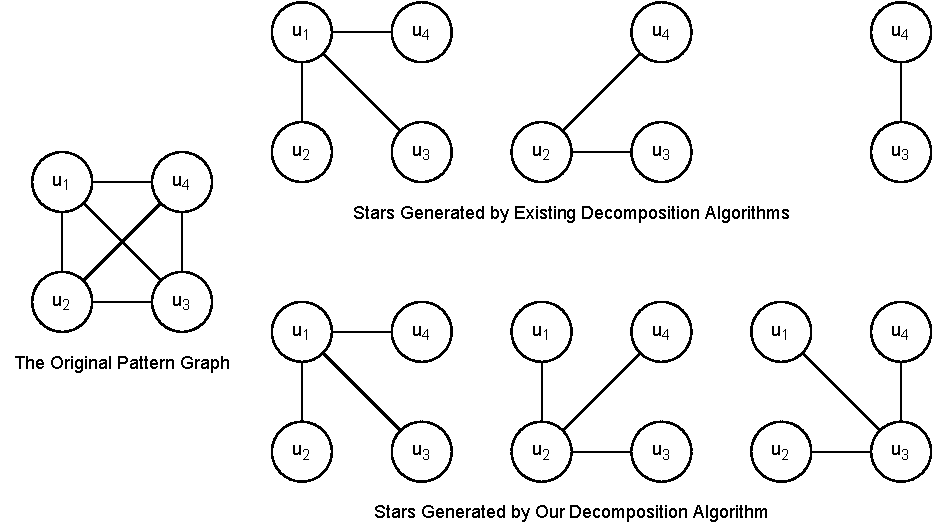
\includegraphics[width=0.48\textwidth]{img/star_decomposition.pdf}
  %%   \caption{Stars decomposed from the same pattern graph using different algorithms.}\label{img:star_decomposition}
  %% \end{figure}
%% \end{enumerate}
\begin{algorithm}[ht]
  \caption{Star decomposition.}\label{alg:decompose_stars}
  \SetKwFunction{DecomposeStars}{\textsc{DecomposeStars}}
  \SetKwFunction{Peek}{\textsc{Peek}}
  \SetKwFunction{Star}{\textsc{Star}}
  \SetKwFunction{RemoveVertex}{\textsc{RemoveVertex}}
  \Fn{\DecomposeStars{$p$}}{
    $stars \leftarrow \emptyset$\;
    $p' \leftarrow p$\;
    $R \leftarrow \{\max_{u \in V(p)}f(u)\}$\;
    \While{$R \neq \emptyset$}{
      $root \leftarrow \max_{u \in R}f(u)$\;
      $R \leftarrow R \setminus \{ root \}$\;
      $R \leftarrow R \cup \{ leaf \mid leaf \text{ is adjacent to } root \text{ in } p'\}$\;
      \RemoveVertex{$p'$, $root$}\;
      $R \leftarrow R \setminus \{ u \mid u \in p' \land \deg{u} = 0 \}$\;
      $stars \leftarrow stars \cup \{$ \Star{$p$, $root$} $\}$\;
    }
    \Return{$stars$}
  }
\end{algorithm}

To match a star $S$ on the vertex-centric storage engine,
SeqStar firstly seeks the \textsc{VertexIter} by searching the global index of the storage engine.
For each vertex $v$ in \textsc{VertexIter},
SeqStar checks the degree of $v$ and applies constraints if available (\S\ref{sec:match_optimize}) to determine whether $v$ could be matched.
If $v$ passes these filters, SeqStar checks the neighbors of $v$ by visiting the \textsc{NeighborIter}.
For each neighbor vertex $n$ in \textsc{NeighborIter},
the in/out-edges associated with $n$ is compared to the corresponding leaf vertex of the star pattern.
The constraints extract from the WHERE clause will be applied to filter out unnecessary $n$ (\S\ref{sec:match_optimize}).
Since the iterators will only incur sequential data accesses,
the star matching process avoids the random disk seeks.

SeqStar adopts two techniques to further reduce the I/O cost:
(1) SeqStar analyzes the isomorphism among the stars to avoid redundant I/Os.
%% Some pattern may generate isomorphic stars, e.g., a triangle where each vertex has an edge point in and out.
Though the general graph isomorphism problem is NP complete~\cite{DBLP:conf/stoc/Cook71}, the isomorphism of stars are much easier to check.
We define an order for the vertices in a star based on the vertex labels. The isomorphism among stars can be checked by comparing the sorted stars.
Isomorphic stars have the same matching results. They only need to match once.
%and SeqStar will only match once for all.
(2) As the disk scanning operation is time consuming, it is preferable to scan it only once when solving a property graph matching problem.
SeqStar addresses the challenge by grouping stars with the same root label together,
and matches them in a single \textsc{VertexIter}.
For each scanned vertex $v$, SeqStar will check all the star patterns with the same root label as $v$.
Therefore, the graph data can be scanned only once without back and forth seeking.

%% Since the real-world graphs are so large that it is preferable to scan it only once when solving a property graph matching problem.
%% SeqStar solves the problem by grouping stars with the same root label together,
%% and scans these stars together by iterating through the \textsc{VertexIter}.
%% For each scanned vertex, SeqStar visits the \textsc{NeighborIter} to check the neighbors and stores the intermediate results for these stars.
%% Moreover, SeqStar is able to find isomorphism among stars and avoids unnecessary star matching (\S\ref{sec:match_optimize}).
%% However, it is not a simple task to match multiple stars in a single sequential scan,
%% the context switch cost and the intermediate result write cost must be minimized.
%% For the context switch cost, it is strongly coupled with the underlying storage method of the data graph.
%% Thanks to the elegant design of our vertex-centric storage model,
%% which is able to match stars in a sequential run given a root label,
%% we could group the stars with the same root label together and match them at the same time when iterating through \textsc{VertexIter}.
%% For the matching result write cost, we developed a compression algorithm for star's matching results that could be wrote sequentially (Section~\ref{sec:match_compress}).
%% As a result, we could scan the huge data graph only once and all the I/Os are sequential.
